\documentclass[12pt]{article}
\usepackage[utf8]{inputenc}
\usepackage{cite}
\usepackage[spanish]{babel}
\selectlanguage{spanish}
\usepackage{graphicx}
\graphicspath{ {files/} }
\usepackage{url}
\usepackage{natbib}




\title{Reporte sobre la Actividad 8}
\author{García Parra Pedro}
\date{Abril 2019}

\begin{document}

\maketitle
Para esta actividad trabajamos con dos archivos de datos simultaneamente: los datos meteorológicos de la estación de Nogal y datos del suelo recolectados en 2009. Primeramente utilic\'e la biblioteca de \textbf{pandas} para leer los archivos y guardar los datos en dataframes, una vez los obtuve prosegu\'i a arreglarlos, esto significa convertir la columna que contenian fechas o datos de tiempo a formatos de fechas ademas de agregar columnas que ser\'an de utilidad como los valores maximos, minimos y promedios de los datos.

En el primer inciso se pide que se grafique la temperatura del aire y del suelo de un solo d\'ia, para ello se requiere cortar los dataframes para obtener otros con solamente un d\'ia de datos; por la forma en la que estan guardados los datos del archivo del suelo fue muy facil partirlo para obtener solo un d\'ia. Para el otro fue un poco m\'as complicado, ya que \'estos eran m\'as (los datos del suelo estaban tomados cada 10 min y los del aire cada 30 min) por lo que pens\'e en promediar los datos cada 30 minutos para as\'i tener la misma cantidad de datos:
\begin{verbatim}
    meteo1dia = []
    hora = []
    n = 0
    suma = 0
    for i in meteo.index:
        if (meteo["DIA"][i] == 1):
            if (n < 3) :
                n += 1
                suma += meteo["airT_Avg"][i]
            else:
                meteo1dia.append(suma/3)
                hora.append(meteo["TIME"][i-1])
                suma = meteo["airT_Avg"][i]
                n = 1
        else:
            suma += meteo["airT_Avg"][i]
            meteo1dia.append(suma/3)
            hora.append(meteo["TIME"][i])
            break
\end{verbatim}
Una vez obtuve estos datos los agreg\'e a un dataframe aparte para poder graficar de una manera m\'as sencilla. Los resultados se muestran en la figura \ref{fig:undia}



La realizaci\'on de el segundo inciso fue f\'acil ya que previamente hab\'ia creado una columna con las temperaturas promedio, maxima y minima diaria, \'esto fue realizado con una serie de groupby:
\begin{verbatim}
    meteo["Tair_AvgDiaria"] = meteo.groupby(["AÑO","MES","DIA"])
                            ["airT_Avg"].transform("mean") 
    meteo["Tair_max"] = meteo.groupby(["AÑO","MES","DIA"])
                            ["airT_Avg"].transform("max")
    meteo["Tair_min"] = meteo.groupby(["AÑO","MES","DIA"])
                            ["airT_Avg"].transform("min") 
\end{verbatim}
De la misma manera se realiz\'o para los datos del suelo, en la figura \ref{fig:aire} se aprecia una de las gr\'aficas que se piden.


A continuaci\'on se nos pide calcular el promedio cada 30 minutos durante el día para el mes de Enero de la temperatura del aire y las 8 temperaturas promedio de subsuelo, para posteriormente graficar la variación en 24 horas de las temperaturas de interés. Como solo utilizaremos 4 temperaturas del suelo y esas ya estaban en el dataframe solamente tom\'e esas en cuenta.
Obtener los datos de enero del dataframe del suelo fue sencillo solamente fue necesario una l\'inea de codigo:
\begin{verbatim}
    SoilEnero = soil[soil["DIA"] <= 31 ]
\end{verbatim}
Esto lo que hace es simplemente agarrar los datos donde el d\'ia es menor igual a 31 as\'i me aseguro de obtener todos los d\'ias de enero, Para el dataframe del aire fue mas complicado, tuve problemas con la forma en la que los datos estaban tomados ya que son muy diferentes a los del suelo (los datos se recolectaban en diferentes tiempos y los d\'ias acaban a diferentes horas) pero finalmente cree un codigo que obtenga el promedio cada 30 minutos y as\'i poder tener la misma cantidad de datos en ambos dataframes.
El codigo que utilic\'e para obtener los datos del aire es el siguiente:
\begin{verbatim}
    mes = 1
    n = 1
    prom = 9.4
    promedios = []
    hora = []
    fecha = []
    indexes = []
    for i in meteo.index:
        if(meteo["MES"][i] == mes): 
            if(n < 3):
                n += 1
                prom += meteo["airT_Avg"][i]
            else:
                promedios.append(prom/n)
                hora.append(meteo["TIME"][i])
                fecha.append(meteo["DIA"][i])
                indexes.append(i)
                prom = meteo["airT_Avg"][i]
                n = 1
        else:
            break
\end{verbatim}
Como los datos comenzaban en el minuto 10 no en el minuto 0 tuve que hacer como si existiera un dato en el tiempo 0 para poder hacer que el algoritmo funcionara de una manera m\'as facil, por eso n comienza en 1 y existe un promedio prom de 9.4 de manera que \'este es el promedio del dato \textit{inventado} 0 con el dato 10.\\
Una vez se obtuvieron \'estos datos fue simple cuestion de graficar, las gr\'aficas se encuentran en las figuras \ref{fig:aireEnero} y \ref{fig:sueloEnero}

\begin{figure}
    \centering
    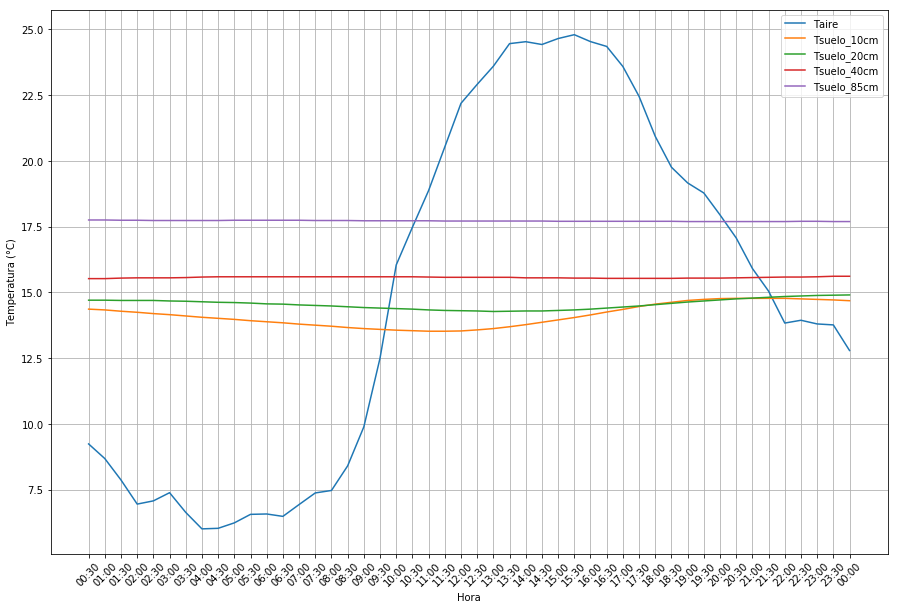
\includegraphics[scale = .4]{undia.png}
    \caption{Datos del dia 1/enero/2009 de la temperatura del aire junto con la temperatura del suelo a diferentes profundidades.}
    \label{fig:undia}
\end{figure}
\begin{figure}
    \centering
    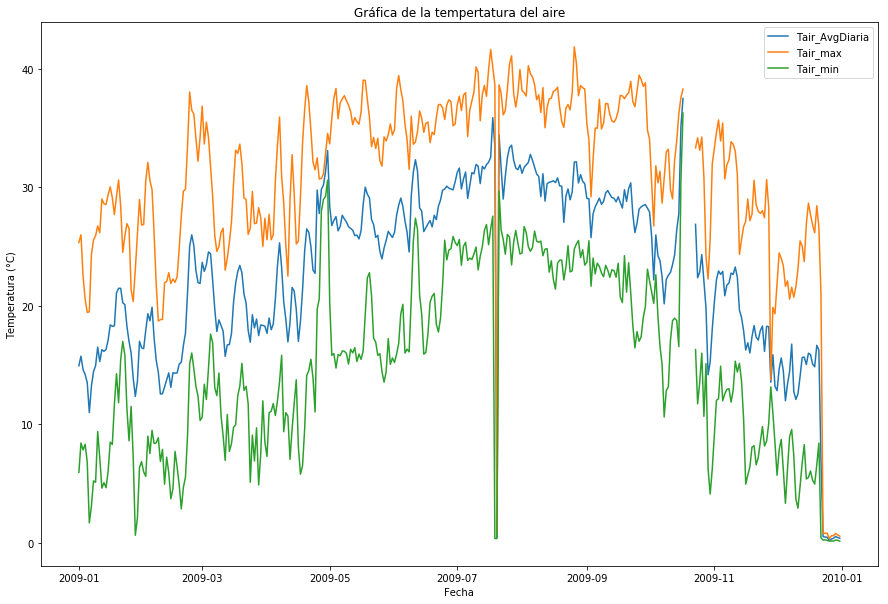
\includegraphics[scale=.4]{aire.png}
    \caption{Gr\'afica de la temperatura promedio, maxima y minima del aire durante todo el año de 2009}
    \label{fig:aire}
\end{figure}
\begin{figure}
    \centering
    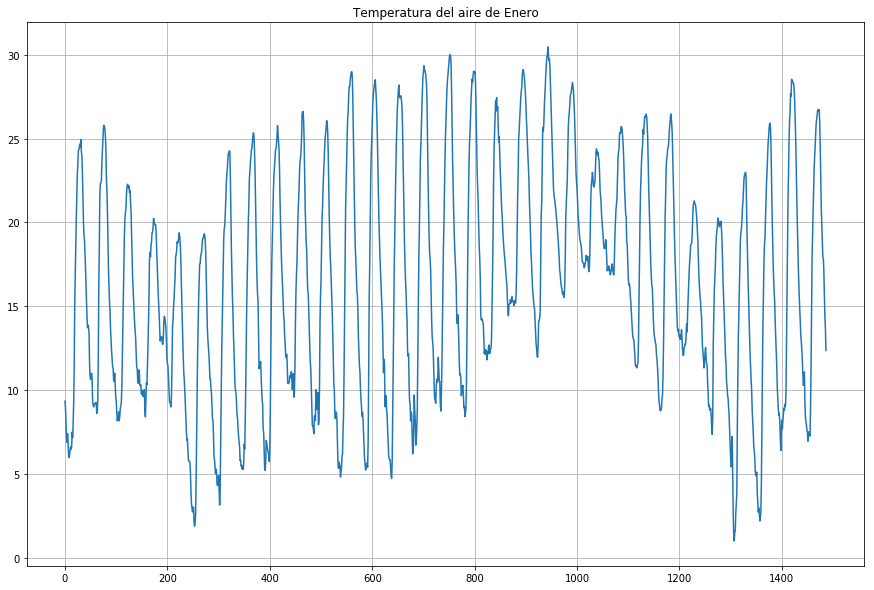
\includegraphics[scale = .4]{aireEnero.png}
    \caption{Grafica de la variaci\'on de la temperatura del aire durante todo el mes de enero del año 2009}
    \label{fig:aireEnero}
\end{figure}
\begin{figure}
    \centering
    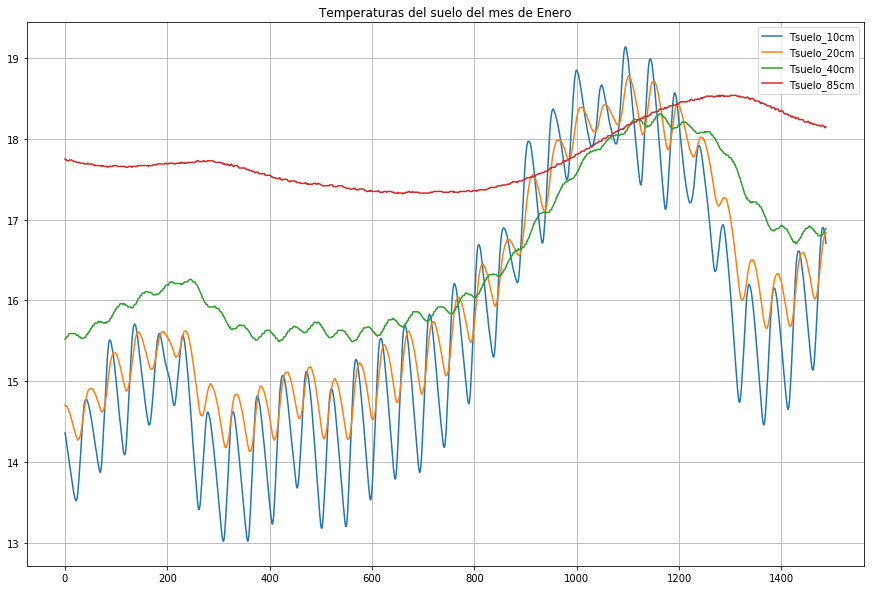
\includegraphics[scale = .4]{sueloEnero.png}
    \caption{Gr\'afica de la variaci\'on de la temperatura del suelo a diferentes profundidades durante todo el mes de enero del año 2009}
    \label{fig:sueloEnero}
\end{figure}
\end{document}
